 \documentclass[a4paper,12pt]{article}
% Margins
\usepackage{a4wide}
% Write english
\usepackage[english]{babel}
% Used for images
\usepackage{graphicx}
% Used to show eps on Windows
\usepackage{epstopdf}
\usepackage{float}
% Text encoding
% Needed to use headers
\usepackage{fancyhdr}
\usepackage{hyperref}
% Used for the euro symbol
\usepackage[gen]{eurosym}
% Used for optimal usage of gensymb4
\usepackage{textcomp}
% Used for the degree symbol
%\usepackage{gensymb}
% Used for captions and subcaptions on images
\usepackage{caption}
\usepackage{subcaption}
% Colors
\usepackage{color}
% Code fragments
\usepackage{listings}

% No tab at start of paragraph
\setlength{\parindent}{0em}
\setlength{\parskip}{1em}

% Defines the todo macro
\newcommand{\todo}[1]{\textcolor{red}{\textbf{TODO: #1}}\PackageWarning{TODO:}{#1!}}

\usepackage{booktabs}% http://ctan.org/pkg/booktabs
\usepackage{colortbl}% http://ctan.org/pkg/colortbl
\usepackage{amsmath}% http://ctan.org/pkg/amsmath
\usepackage{xcolor}% http://ctan.org/pkg/xcolor
\usepackage{graphicx}% http://ctan.org/pkg/graphicx

\colorlet{tableheadcolor}{gray!25} % Table header colour = 25% gray
\newcommand{\headcol}{\rowcolor{tableheadcolor}} %
\colorlet{tablerowcolor}{gray!10} % Table row separator colour = 10% gray
\newcommand{\rowcol}{\rowcolor{tablerowcolor}} %
    % Command \topline consists of a (slightly modified) \toprule followed by a \heavyrule rule of colour tableheadcolor (hence, 2 separate rules)
\newcommand{\topline}{\arrayrulecolor{black}\specialrule{0.1em}{\abovetopsep}{0pt}%
            \arrayrulecolor{tableheadcolor}\specialrule{\belowrulesep}{0pt}{0pt}%
            \arrayrulecolor{black}}
    % Command \midline consists of 3 rules (top colour tableheadcolor, middle colour black, bottom colour white)
\newcommand{\midline}{\arrayrulecolor{tableheadcolor}\specialrule{\aboverulesep}{0pt}{0pt}%
            \arrayrulecolor{black}\specialrule{\lightrulewidth}{0pt}{0pt}%
            \arrayrulecolor{white}\specialrule{\belowrulesep}{0pt}{0pt}%
            \arrayrulecolor{black}}
    % Command \rowmidlinecw consists of 3 rules (top colour tablerowcolor, middle colour black, bottom colour white)
\newcommand{\rowmidlinecw}{\arrayrulecolor{tablerowcolor}\specialrule{\aboverulesep}{0pt}{0pt}%
            \arrayrulecolor{black}\specialrule{\lightrulewidth}{0pt}{0pt}%
            \arrayrulecolor{white}\specialrule{\belowrulesep}{0pt}{0pt}%
            \arrayrulecolor{black}}
    % Command \rowmidlinewc consists of 3 rules (top colour white, middle colour black, bottom colour tablerowcolor)
\newcommand{\rowmidlinewc}{\arrayrulecolor{white}\specialrule{\aboverulesep}{0pt}{0pt}%
            \arrayrulecolor{black}\specialrule{\lightrulewidth}{0pt}{0pt}%
            \arrayrulecolor{tablerowcolor}\specialrule{\belowrulesep}{0pt}{0pt}%
            \arrayrulecolor{black}}
    % Command \rowmidlinew consists of 1 white rule
\newcommand{\rowmidlinew}{\arrayrulecolor{white}\specialrule{\aboverulesep}{0pt}{0pt}%
            \arrayrulecolor{black}}
    % Command \rowmidlinec consists of 1 tablerowcolor rule
\newcommand{\rowmidlinec}{\arrayrulecolor{tablerowcolor}\specialrule{\aboverulesep}{0pt}{0pt}%
            \arrayrulecolor{black}}
    % Command \bottomline consists of 2 rules (top colour
\newcommand{\bottomline}{\arrayrulecolor{white}\specialrule{\aboverulesep}{0pt}{0pt}%
            \arrayrulecolor{black}\specialrule{\heavyrulewidth}{0pt}{\belowbottomsep}}%
\newcommand{\bottomlinec}{\arrayrulecolor{tablerowcolor}\specialrule{\aboverulesep}{0pt}{0pt}%
            \arrayrulecolor{black}\specialrule{\heavyrulewidth}{0pt}{\belowbottomsep}}%
\begin{document}
\begin{titlepage}
\fontsize{12pt}{14pt}\selectfont

\begin{center}
% The logo of the University of Ghent

\includegraphics[height=4cm]{figures/logo}

\vspace{1cm}

\fontsize{14pt}{17pt}\selectfont
% The course:
\textsc{Advanced Multimedia Applications}
\fontsize{12pt}{14pt}\selectfont
\vspace{1.5cm}

% De auteur van de thesis:
Feliciaan De Palmenaer\\
Wouter Pinnoo\\
Stefaan Vermassen\\
Titouan Vervack

\vspace{2.8cm}

\fontsize{17.28pt}{21pt}\selectfont

% The title:
\textsc{Academic Data - Automatic Course Assembly}
\fontseries{m}
\fontsize{12pt}{14pt}\selectfont

\vspace{3cm}
2015-2016
\vspace{2cm}

\end{center}
\end{titlepage}
\thispagestyle{empty}

\tableofcontents
\newpage
% ---------------------------------------------------------------------------- %
%                                  Titlepage                                   %
% ---------------------------------------------------------------------------- %

% ---------------------------------------------------------------------------- %
%                                     Body                                     %
% ---------------------------------------------------------------------------- %
\fontsize{12pt}{16pt}\selectfont

\section{General Information}
Onsophic, a Silicon Valley based startup focused on transforming learning, offers an intuitive, data driven, online training platform. The platform continuously gathers and analyses learning data and can
therefore be seen as the equivalent of Google Analytics for learning by providing organizations with a toolset to measure, analyse and discover what works and, more importantly, what doesn't work in training. In this business process, integrating existing content into the e­-learning
platform is crucial.
The goal in this project is to automate the course assembly process, by transforming raw learning materials into structured courses.
\section{General project decisions}
This section will outline all of the important decisions we have made during the development of the project.
\subsection{Decisions}
\textbf{Iteration 1 (Course introduction - 18/02/2016)}
\begin{itemize}
    \item Stefaan will fulfil the role of team lead. (18/02)
    \item Stefaan will be responsible for the communication with the other parties. (18/02)
    \item Git will be used as distributed versioning control system for the code, with the UGent GitHub platform as tool. (20/02)
    \item Titouan will be responsible for the progress report and will make sure it is always up to date. (22/02)
    \item Wouter will be responsible for git and over the code quality. (22/02)
    \item Feliciaan will be responsible for the planning of the project. (22/02)
   \item For scalability purposes, a web service is chosen over a native application (22/02)
\end{itemize}
\textbf{Iteration 2 (Starting 24/02/2016)}
\begin{itemize}
   \item Play web application framework is chosen. Play is written in Scala and Java and is a clean alternative to the legacy Enterprise Java stacks focusing on predictable, minimal resource consumption (25/2)
    \item Akka is chosen to create the asynchronous task system. Akka is a toolkit and runtime for building highly concurrent, distributed, and resilient message-driven applications on the JVM (25/2)
    \item For Named-Entity Recognition, the NERD API was chosen for its abstraction of other NER APIs. (25/2)
    \item We chose to use jsoup for our HTML parser as it doesn't require us to create the syntax tree ourselves and because it implements the WHATWG HTML5 specification. This on it's own, using ANTR4, would take quite some time. The license used for jsoup is the MIT license, strengthening our choice. (25/2)
\end{itemize}
\textbf{Iteration 3 (Starting 09/03/2016)}
\begin{itemize}
   \item To decrease the impact of the risk \textit{``NER processing is not fast enough for practical usage of our tool"}, use several NER services in parallel and only choose the fastest one (12/03)
   \item Implement threading for parallel processing of the several documents that have to be recognised in one task (12/03)
\end{itemize}
\textbf{Iteration 4 (Starting 16/03/2016)}
\begin{itemize}
 \item We have defined a set of supported input formats. We noticed that most user manuals come with a Toc. The web service will expect this Toc only, and will dynamically decide which formatting is used (nested unordered lists, nested tables, divs,..). 
 \item Error handling implementation
 \item Get partial JSON before NER to avoid long wating times before any result

 \item Chapters are meant to group modules, no other metadata is attached to a chapter. Chapters are optional. So if you are able to detect an extra level on top of modules, you can use chapters to reflect that extra level.
\item  The only tags that matter for now are the section tags, so we only focus on these.
\end{itemize}

\subsection{Responsibilities}
\begin{tabular}{lp{12cm}}
  \topline
  \headcol Responsible & Task  \\
  \midline
\textbf{Iteration 2} \\\\
 \rowcol Titouan & - Responsible for the initial architecture\\
 \rowcol & - Digitalising the component-connector diagram \\
 \rowcol & - Initial wireframe of classes \\
 Feliciaan & - Library research for input parsing\\ 
 & - Adding HTML parser to the solution \\
 & - Handle multiple URLs \\
 \rowcol Wouter & - Research on Named-Entity Recognition libraries\\ 
\rowcol  & - Making a motivated decision on which NER tool or tools are most suitable for what you need, and which will be the easiest to integrate into the solution, and be most future-proof \\
\rowcol & - Implement the most optimal solution for NER.\\ 
Stefaan & - Setting up the initial Play project\\ 
 & - Creating an asyncronous task system using Akka to come up with a scalable approach \\
 & \\\hline
\textbf{Iteration 3} \\\\
 \rowcol Titouan & - Implement threading (parallel functionality for different documents in the same task)\\
 Feliciaan & - Use the parsed HTML document to fill in section names in the Onsophic JSON document\\
 \rowcol Wouter & - Risk list, planning and presentation\\ 
Stefaan & - Research on Onsophic JSON format, progress report\\
 & \\\hline
\textbf{Iteration 4} \\\\
  \bottomlinec
\end{tabular}
\subsection{Requirements}
\subsubsection{Functional requirements}
\textbf{Must-haves}
\begin{itemize}
    \item parse the input source (HTML)
    \item detect the learning modules and their learning activities
    \item tag these detected modules and activities based on named entity recognition
    \item estimate the Bloom level for each of the detected activities
\end{itemize}
\textbf{Nice-to-haves}
\begin{itemize}
    \item Detect chapters in the HTML document, as these are optional (property of a module).
    \item Parse other types of documents than use manuals.
\end{itemize}
\subsubsection{Non-functional requirements}
\textbf{Must-haves}
\begin{itemize}
    \item Interoperability. Our tool must be able to interchange information with third-party services correctly. See Quality-Attribute Scenario in Figure \ref{fig:qas-interoperability}.
    
\begin{figure}[H]
  \centering
      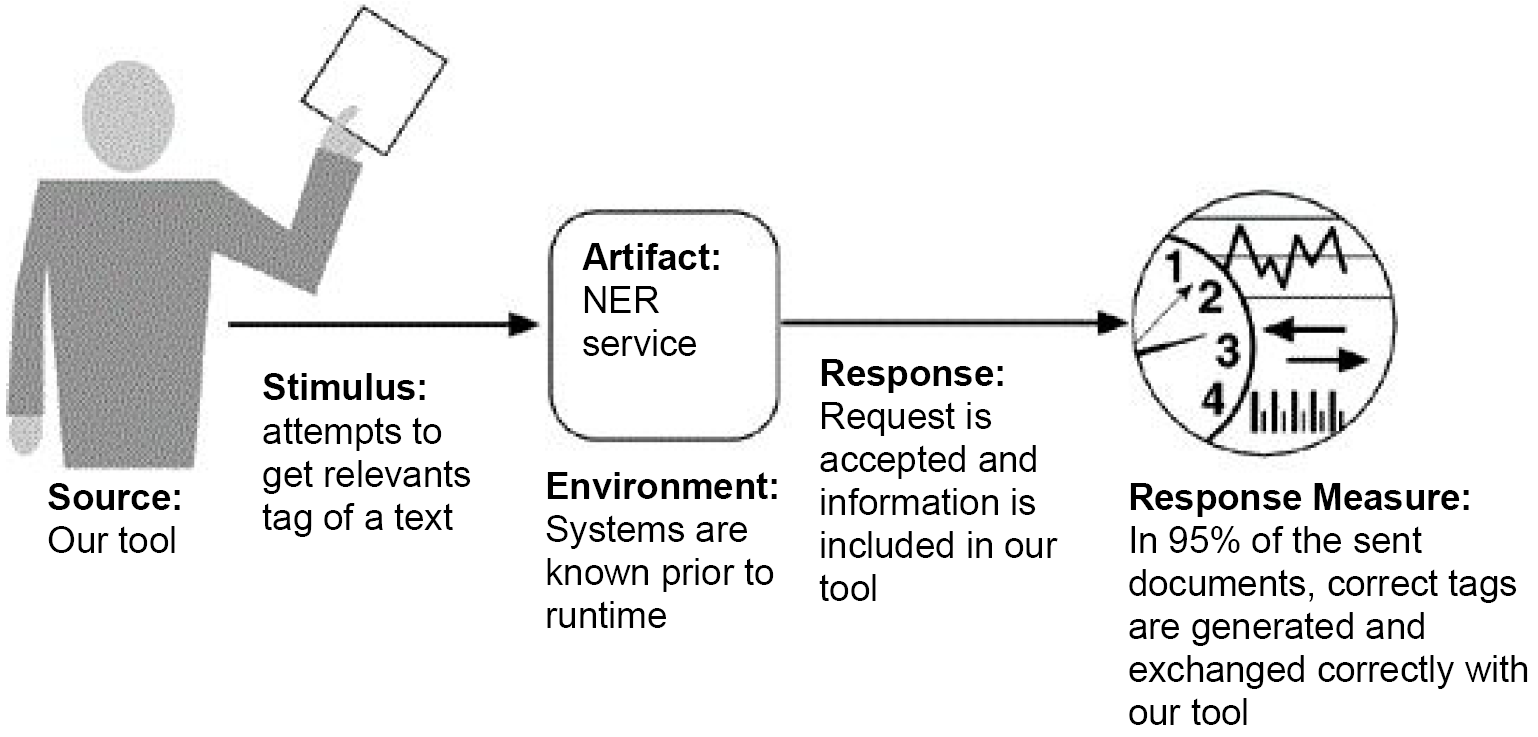
\includegraphics[width=0.9\textwidth]{figures/QAS-interoperability}
  \caption{QAS: interoperability}
\label{fig:qas-interoperability}
\end{figure}

    \item Modifiability. A developer must be able to change formats of input/output documents without it having an impact on other modules. See Quality-Attribute Scenario in Figure \ref{fig:qas-modifiability}.
    
\begin{figure}[H]
  \centering
      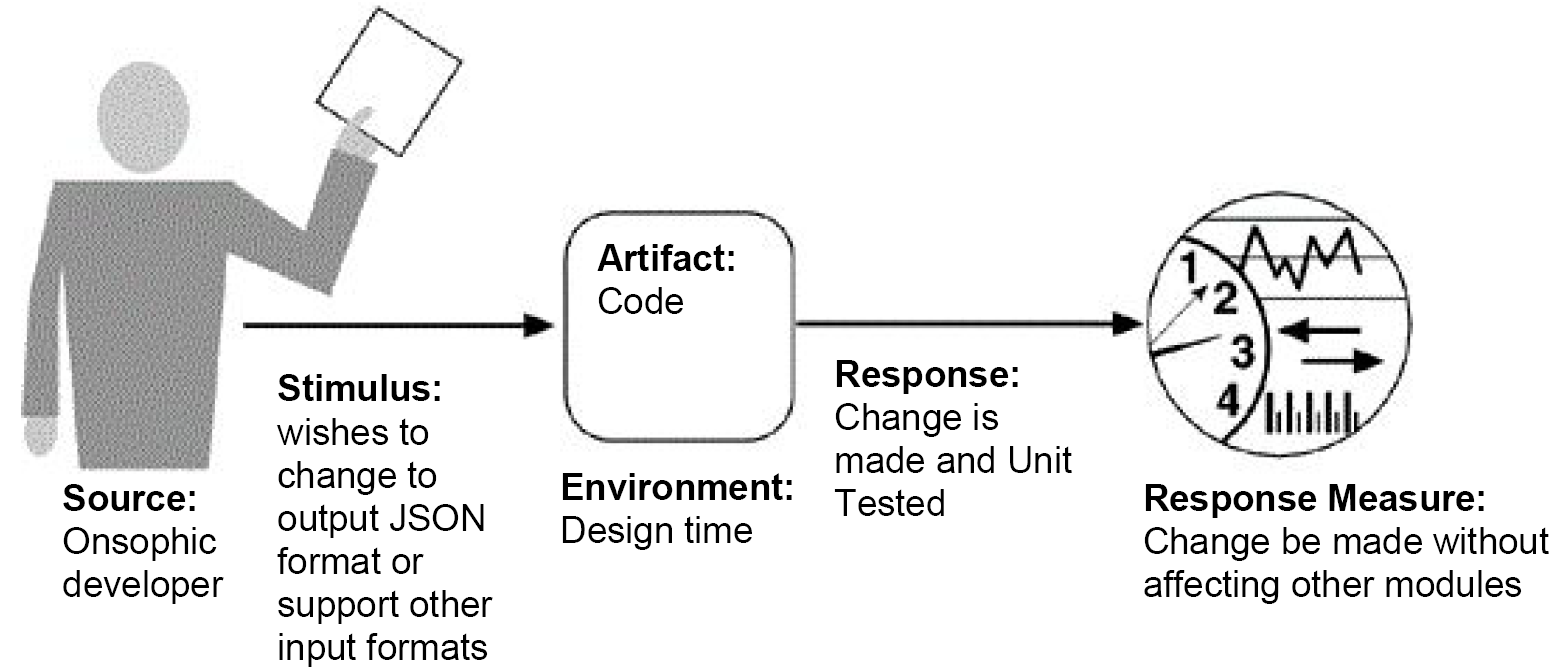
\includegraphics[width=0.9\textwidth]{figures/QAS-modifiability}
  \caption{QAS: modifiability}
\label{fig:qas-modifiability}
\end{figure}
    
\end{itemize}
\subsection{Assumptions}
\subsubsection{Input}
After surveying multiple different helpsites we didn't find any similarities that worked for all sites.
Some sites can be parsed by counting the depth of the node in the parse tree.\\
Some sites have a first page which is the index, other sites have the index on every page, some even need use javascript to create the whole index of the site.\\

At the moment we have implemented our parser for sites that have a table of contents.\\
We assume that every html document contains exactly one document.
\subsection{Risk list}
\begin{tabular}{p{5.5cm}llp{5.5cm}}
  \topline
  \headcol Risk & Probability & Impact & Mitigation  \\
  \midline
 \rowcol Not finding a generic line in the different input sources & M & H & Review the assumptions about the input data with the client\\
No suitable NER tool that is free to use and license to use in closed-source software & L & H & Looking into commercial tools\\
 \rowcol Time-management issues due to other projects and master dissertation & M & M & Discuss planning and requirements with client\\
 NER processing is not fast enough for practical usage of our tool & M & M & Use several services in parallel and only use the fastest one\\
 \rowcol Not able to fill in all metadata (not fully compatible JSON) & H & L & Use simplified JSON\\
  \bottomlinec
\end{tabular}
\subsection{APIs \& frameworks}
\begin{enumerate}
\item Play Framework: web application framework, written in Scala and Java, clean alternative to the legacy Enterprise Java stacks, focussing on predictable, minimal resource consumption
\item Akka: toolkit and runtime for building highly concurrent, distributed, and resilient message-driven applications on the JVM
\item For the parsing of HTML we use jsoup. It implements the WHATWG HTML5 specification and creates the same DOM (Document Object Model) as modern browsers create.
\item Named-Entity recognition will be done using the NERD API.
\end{enumerate}
\section{Prototype}
\subsection*{Iteration 2 (Starting 24/02/2016)}
\subsubsection*{Architecture}
\begin{figure}[H]
  \centering
      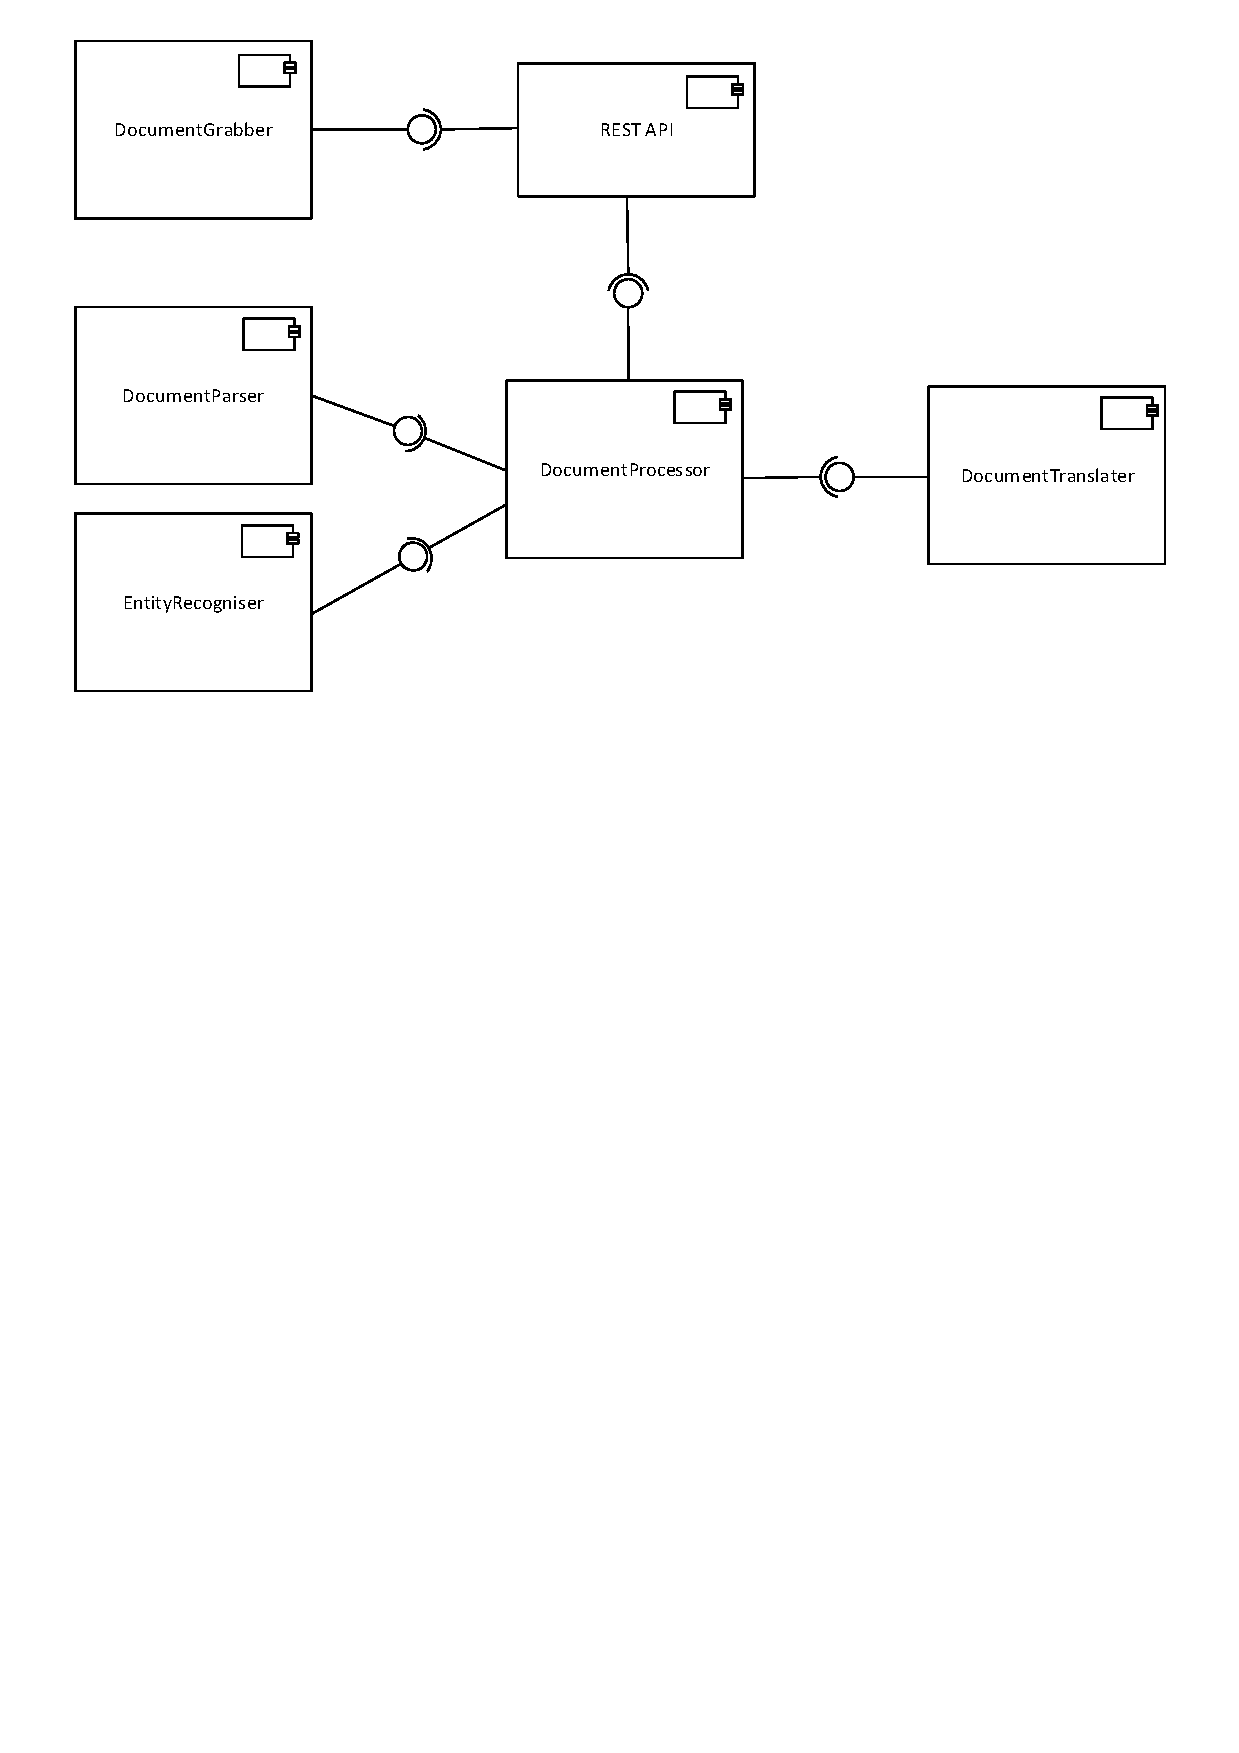
\includegraphics[width=0.9\textwidth]{design/components}
  \caption{Initial high-level architecture of the Automatic Course Assembly service}
\label{fig:intelligence}
\end{figure}
Our initial architecture is modular and has as goal to easily allow to extends our application with more features later on. Adding a new type of input or output format for example should be as easy as possible.\\

First and foremost we have the REST API, this is the starting points of our application. A url will be passed to our REST API after which it will use the right DocumentGrabber to grab the document from the url. An example of a DocumentGrabber would be an HTMLGrabber that knows how to grab HTML documents and returns an unprocessed HTMLDocument.\\
Throughout the application we will work with Documents to pass around the (un)processed data.\\
The REST API then passes the Document it grabbed to the DocumentProcessor. The Processor calls the DocumentParser which will create a parse tree, analyse it and create a new Document, during analysis the learning modules and activities are created. In this Document only the useful parts of the input document are left over.\\
The DocumentProcessor than passes the parsed Document to the EntityRecogniser which will perform Named Entity Recognition (NER) on the Document. This module will add tags to the Document and pass it back to the DocumentProcessor.\\
Last but not least the DocumentProcessor passes the Document to a DocumentTranslator which will translate a completely processed Document into a Document fit for outputting. In our current case, this will translate an HTMLDocument into a JSONDocument.\\

The only document that can be accessed from the outside is the REST API, everything else is hidden from the user. The user can query the API to start a new import, get the status of a previous task or get the generated output document.
\subsubsection*{NER}
In the assembly process of the JSON-representation of a course document, tags will be created in addition to the parsed content of the (HTML-) documents. For each document, these tags will represent the subject of the document. For this purpose, the content of the whole document will have to be scanned, since the title of the document is not always sufficient to serve as tag for the document. For example, user manuals often contain \textit{Prerequisites} as a title for the first section of the manual. This section will probably contain more useful information than only this subject line.\par
For the automatic scanning of the document for useful tags, Named-Entity Recognition (NER) will be used. NER uses machine learning techniques to find (sequences of) words in the text, i.e. entities, that can be related to concepts from the semantic web. For example, in the sentence \textit{Trump and Clinton are two candidates for the presidential elections of 2016}, the entity \textit{Trump} will be linked to \textit{http://dbpedia.org/page/Donald\_Trump}. The used algorithm will make decisions based on relevance of the word to the concept of the semantic web and its confidence.\par
We think NER is the best solution for the generation of tags, since
\begin{itemize}
\item NER finds sequences of words that are relevant (i.e. leave out words like \textit{'and'}, \textit{'or'}, \textit{'the'}, etc.
\item NER provides a measure of relevance, which we can use to sort all entities on. Only the 5 most relevant concepts in the document will be used as tag for the document.
\end{itemize}\par
Several NER libraries exist that serve an API for easy access. We chose to use the NERD API\footnote{see http://nerd.eurecom.fr/}. This API acts as an abstraction layer for other existing NER APIs, one of which is the most commonly used NER API: AlchemyAPI. The NERD API provides easy methods to submit a document, choose a NER library and retrieve the results of the chosen extractor.\par
This abstraction layer will be a big advantage in this project, because we can easily switch from extractors to tune performance and correctness of the tags.\par
A disadvantage of the NERD API is its license, which prohibits any commercial use of its services. However, we think that the benefit of the abstraction layer outweighs the disadvantage of the license, since one can use the learned results of all the different used extractors gained in this project course to eventually implement the best performing extractor in the project (which will take more effort than implementing this abstraction layer).\par

\subsection*{Demo}
\begin{itemize}
\item Entering new URL in the system:
\begin{lstlisting}
$ http http://localhost:9000/start\ 
?url=https://docs.oracle.com/cd/E18727_01/doc.121/e13522/toc.htm
HTTP/1.1 200 OK
Content-Length: 27
Content-Type: application/json; charset=utf-8
{
    "id": 1,
    "status": "QUEUED"
}
\end{lstlisting}
\item Checking progress of a task
\begin{lstlisting}
$ http localhost:9000/check?id=1
HTTP/1.1 200 OK
{
    "id": 1,
    "status": "RECOGNISING"
}
\end{lstlisting}
\item Retrieving the results of a task
\begin{lstlisting}
$ http localhost:9000/result?id=1
HTTP/1.1 200 OK
{
    "tags": ["tag1", "tag2"],
    "text": "..."
}
\end{lstlisting}
\end{itemize}
\begin{figure}[H]
  \centering
      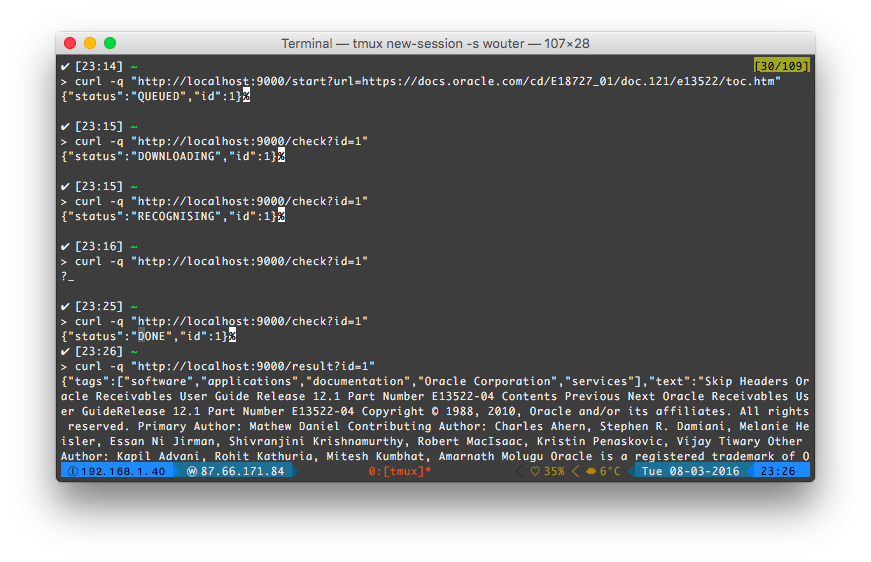
\includegraphics[width=\textwidth]{figures/screenshot-queueing}
  \caption{Screenshot of the queueing process}
\label{fig:screenshot-queueing}
\end{figure}
\subsection*{Iteration 3 (Starting 09/03/2016)}

\subsubsection*{Architecture}
\begin{figure}[H]
  \centering
      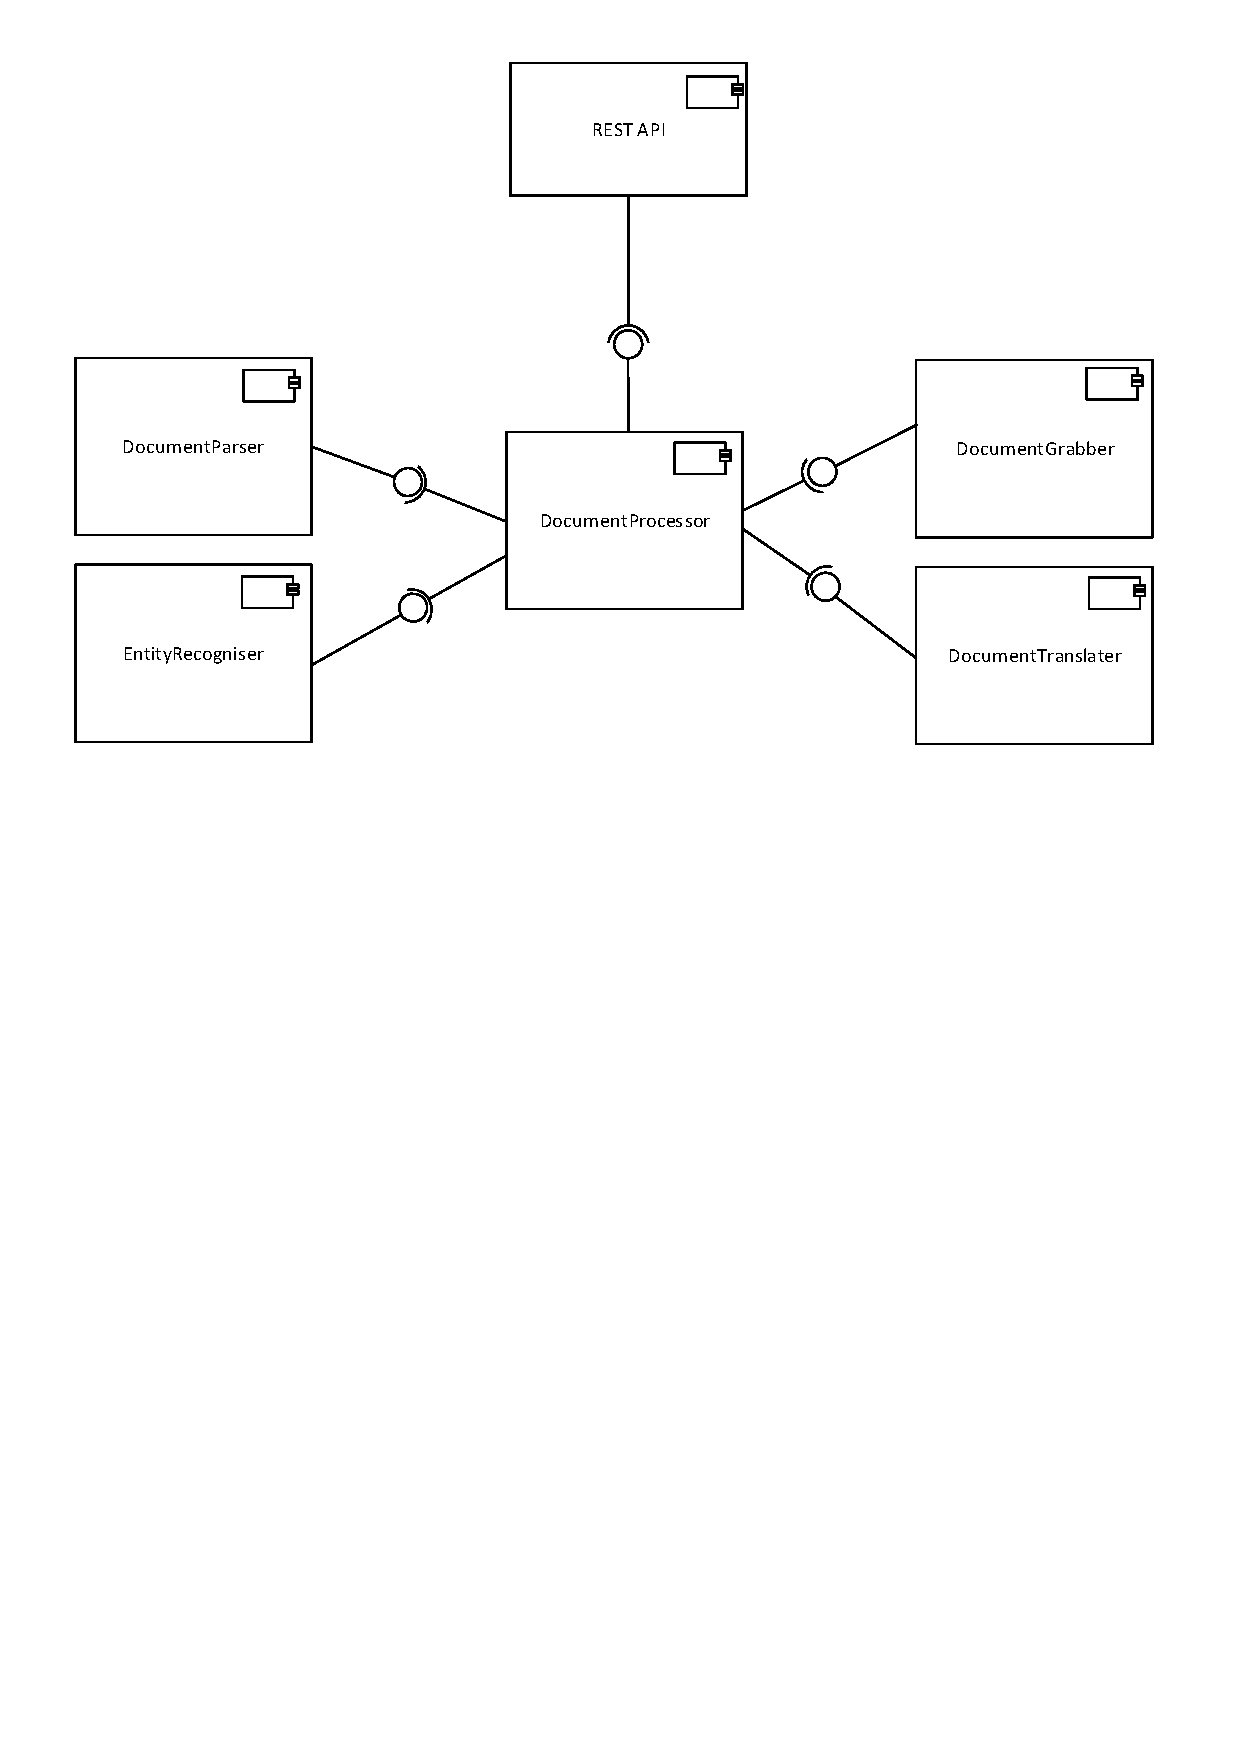
\includegraphics[width=0.9\textwidth]{design/componentsv2}
  \caption{Revised high-level architecture of the Automatic Course Assembly service}
\label{fig:intelligence}
\end{figure}

A few changes were made in this iteration because we noticed that the document we receive as input has links to other documents that should also be grabbed and parsed.\\

In our second architecture the DocumentGrabber has moved to the DocumentProcessor. The API just passes the url of the first url to the DocumentProcessor.\\
In the DocumentGrabber two new thread are created, one in which the DocumentGrabber grabs new documents and one in which the DocumentParser parses the grabbed Document. In the latter more urls can be derived from the document and these are added to the list of documents to grab.\\

The EntityRecogniser and DocumentTranslator remain the same but they are called once for every document that went through the parser.

\subsubsection*{Retrieve section headers}
As a first attempt in parsing, section headers from a HTML manual document were retrieved. Those headers are used in the \verb|embeddedSections|-\verb|title| field in the JSON format of Onsophic, and the tags (retrieval implementation made in iteration 2) are used in the corresponding JSON field. The code below shows the output of our tool at the end of this iteration.
\begin{lstlisting}
$ http localhost:9000/result?id=1
HTTP/1.1 200 OK
{
    "@type":"CourseEdit",
    "title":"AMMA test course",
    "embeddedSections":[
        {
            "@type":"SectionEdit",
            "title":"Oracle Receivables User Guide",
            "activity":{
                "url":"https://docs.oracle.com/cd/E18727_01/doc.121
                       /e13522/toc.htm",
                "modality":"text",
                "activityType":{
                    "id":"READ",
                    "title":"Read"
                },
                "title":"Oracle Receivables User Guide"
            },
            "tags":[
                "Receipts",
                "Transactions",
                "Bills Receivable",
                "Customer",
                "Receivables"
            ],
            "visible":true,
            "optionality":"required"
        },
        {
            "@type": "SectionEdit",
            "title": "...",
            ...
        }
    ]
}
\end{lstlisting}

\subsection*{Iteration 4 (Starting 16/03/2016)}
We have defined a set of supported input formats. We noticed that most user manuals come with a table of contents. The web service will expect this table of contents only, and will dynamically decide which formatting is used (nested unordered lists, nested tables, divs,..). 
\par
As Onsophic indicated that they would like to test the service during the development to give more feedback and evaluate the integration in the learning platform, we decided to expose stable versions of this web service on a web server. For this purpose, an Azure web service has been created that always reflects the stable version on the master branch and is accessible on the following endpoint: \textbf{http://13.94.197.112:9000}.
\par
The supported input formats will be explained in detail in the sections below. For each format, an example is provided.
\subsubsection*{HTML unordered lists}
The table of content lists all the sections in the form of a nested unordered list.
\begin{lstlisting}
<ul>
    <li>List item one</li>
    <li>List item two with subitems:
        <ul>
            <li>Subitem 1</li>
            <li>Subitem 2</li>
        </ul>
    </li>
    <li>Final list item</li>
</ul>
\end{lstlisting}
Example: \url{http://13.94.197.112:9000/assets/examples/lists.html}.
\begin{lstlisting}
 Optional<Element> toc = document.getHtmlDocument()
.select("ul").stream().filter(l -> !l.parent().tag().equals("li"))
.sorted((e1, e2) -> 
    e1.childNodes().size() > e2.childNodes().size() ? -1 : 1).findFirst();
\end{lstlisting}
To find the table of contents on the page, we first get all the lists that are not nested inside another list. The list with most childnodes will be selected. Each child in the parent list will be treated as a Module. If it seems that a Module node has no children, an Section and Activity with the same name will be created artificially. The URL of the activity will represent the URL of the Module node. 
\begin{lstlisting}
//No sublevels found, create new activity with this element's content
//If there is a link assigned to this listelement
if (!e.select(":root > a").isEmpty() && 
    !e.select(":root > a").get(0).attr("href").isEmpty()) {
       Section section = new Section();
       Element linkElement = e.select(":root > a").get(0);
       section.setTitle(linkElement.ownText());
       setActivity(linkElement, section);
       module.addSection(section);
}
\end{lstlisting}


However, as lists can be nested, the children of the Module nodes will be treated as sections. If the Section node has no children, an activity node will be created artificially. The children of Section nodes will be treated as activities.
\subsubsection*{Description lists}
The table of content lists all the sections in the form of a description list.
\begin{lstlisting}
<dl>
  <dt>Firefox</dt>
  <dt>Mozilla Firefox</dt>
  <dt>Fx</dt>
  <dd>A free, open source, cross-platform, graphical web browser
    developed by the Mozilla Corporation and hundreds of volunteers.</dd>

</dl>
\end{lstlisting}
Example: \url{http://13.94.197.112:9000/assets/examples/definitionlists.html}.
\subsubsection*{Raw weblinks}
The table of content lists all the sections in the form hyperlinks. The parser will automatically follow each link and parse the pages on the deeper levels.
\begin{lstlisting}
<a href="http://help.apple.com/ipad/5/voiceover/en/iPad73fccd85.html" 
alt="At a Glance" class="voiceoverListLink">At a Glance</a><br />
<a href="http://help.apple.com/ipad/5/voiceover/en/iPad741db878.html" 
alt="Getting Started" class="voiceoverListLink">Getting Started</a><br />
<a href="http://help.apple.com/ipad/5/voiceover/en/iPad743b0e91.html" 
alt="Basics" class="voiceoverListLink">Basics</a>
\end{lstlisting}
Example: \url{http://13.94.197.112:9000/assets/examples/rawlists.html}.
\subsubsection*{Error handling}
Since we decided that the parsing will be handled asynchronously, it is possible that an error occurs of which the web service consumer doesn't know about. Therefore, we implemented better error handling. If an unhandled exception occurs in the parsing process, this will be visible for the consumer as the error message will now be shown in response of the check method.  \par
Before this implementation, the status of a task would not change and the consumer could wait forever.
\subsubsection*{NER after writing out the JSON}
As the NER lookup is the slowest operation in the process, we decided to make the JSON result accessible before the NER is completed. As soon as the parsing part is done, querying the \verb|result| endpoint will result in the status \verb|DONE_WITHOUT_TAGS|. The returned JSON document will be complete except that the tags array will be empty. As soon as the NER processing is done, the tags array will be filled and the status will be \verb|DONE_WITH_TAGS|.
\subsubsection*{Prefix handling}
We encountered some problems with documents that contain relative links to other documents. Instead of having to modify all links in a document before submitting it to the system, the prefix of the links can be passed to the system in the \verb|start| endpoint. For example, using \verb|?prefix=http://example.com/| will make sure that relative links (e.g. \verb|subpage/page1.html/|) are retrieved correctly.\par
In case no prefix is provided in the \verb|start| endpoint, a prefix will be automatically generated based on the URL of the page that contains the table of contents. For example, submitting \verb|http://example.com/subpage/toc.html| without \verb|prefix| parameter will cause the system to use the prefix \verb|http://example.com/subpage/|.
 
\section{Application}
The application we create is a web API that takes a url of an HTML document. The document is then processed and a JSON document compatible with the JSON format used in Onsophic is created. Multiple requests can be issued simultaneously and the status of a document can also be queried.
\section{Overview of the different meetings}
\subsection{Initial meeting with client (24/02/2016)}
\begin{itemize}
\item \textbf{Present:} Stefaan, Titouan and Wouter
\item \textbf{Excused:} Feliciaan
\item \textbf{Goal:} Getting to know the specific details and requirements for the project.
\item \textbf{Meeting notes:} We met with Davy, the CTO of Onsophic. Onsophic has  seven employees, of which two to three are technical employees. The platform that Onsophic produces is an educational platform, aimed at different companies such as: software, retail,\ldots They are based in Europe \& the USA.\\
The platform offers courses and learning activities. A course exists of modules, each module contains learning activities, e.g. youtube clip, drive document,\ldots. Onsophic hosts nothing by itself, everything is hosted somewhere else.
Documents that have to be imported into the platform are for example user manuals about products. The support can than learn more about the products through the courses. We have to convert our input documents to a series of modules and learning activities.
\item \textbf{Decisions:} This week we received a sample JSON file and test logins for the Onsophic platform. We will have a meeting with the client weekly, the day before meeting with the teaching staff.
\end{itemize}
\subsection{Review with teaching staff (25/02/2016)}
\begin{itemize}
\item \textbf{Meeting notes} 
Make sure to discuss these topics next time:
\begin{itemize}
\item Overview of architecture
\item Who is doing what
\item Risk list
\item What can go wrong, what problems do you have to tackle first, prioritize
\item What features are we going to offer
\item Use your client
\item Include assumptions about inputs in the report!
\item Agile approach, get a demo ready as fast as possible
\item Planning in a powerpoint, what technologies to work together 
\end{itemize}
\item \textbf{Decisions:} Next time, come up with a presentation that gives a summary of the above subjects.
\end{itemize}
\subsection{Review with teaching staff (10/03/2016)}
\begin{itemize}
\item \textbf{Meeting notes:}
\begin{itemize}
\item Define more risks. Not only encountered events, but also risks of events that may happen in the future.
\item Make sure a good planning for the next six weeks is defined and presented on the next meeting (17/03/2016).
\end{itemize}
\end{itemize}


\subsection{Review with client (16/03/2016)}
\begin{itemize}
\item \textbf{Meeting notes:} 
\begin{itemize}
\item An external NER service can be down. Think about mitigations for this risk.
\item Think about possibilities to use our system in a more user-friendly way.
\end{itemize}
\end{itemize}


\subsection{Review with teaching staff (17/03/2016)}
\begin{itemize}
\item \textbf{Meeting notes:} 
\begin{itemize}
\item A more detailed sprint planning must be added to the progress report.
\item A self-reflection on the proposed sprint must be discussed during the next meeting.
\end{itemize}
\end{itemize}



\subsection{Extra internal meeting (28/03/2016)}
\begin{itemize}
\item \textbf{Meeting notes:} 
\begin{itemize}
\item Several sources were researched, and a categorisation is made to
\begin{enumerate}
\item sources with navigation based on simple HTML list tags;
\item sources with navigation places in HTML tables;
\item sources with raw (hierarchical) links.
\end{enumerate}
\end{itemize}
\item \textbf{Decisions:} 
\begin{itemize}
\item Stefaan implements a parser based on category 1.
\item Titouan implements a parser based on category 2.
\item Wouter implements a parser based on category 3.
\item Feliciaan implements the detection of each category and executes the corresponding parser.
\end{itemize}
\end{itemize}



\subsection{Review with client (30/03/2016)}
\begin{itemize}
\item \textbf{Meeting notes:} 
\begin{itemize}
\item There're a lot of possible formats. Make a list of the format we want to support and provide some examples for it.
\item The parsing algorithm should be described more with all relevant constraints.
\item Sometimes a \textit{parent} in the hierarchical tree has content too. In that case, make a separate section that contains that content, e.g. an \textit{``Introduction"} section.
\item Make a better error handling system, where a user gets notified it things go wrong.
\item Units are not yet implemented. Without units, we can not import our JSON into the client's system.
\item Both \textit{Bloomlevels} and \textit{Modalities} have to be implemented.
\end{itemize}
\item \textbf{Decisions:} 
\begin{itemize}
\item Stefaan provides the client with a link to the Azure production server.
\item Wouter checks whether the used NER service has a usage limitation.
\item The client provides the team with correct user permissions on his platform.
\end{itemize}
\end{itemize}


\subsection{Review with client (13/04/2016)}
\begin{itemize}
\item \textbf{Meeting notes:} 
\begin{itemize}
\item The proposed categorisation of Bloomlevels is too wide. The client will provide the team with the exact list of keywords that will have to be used in the application.
\item Testing is not yet possible because there was an error while deploying on Azure. This will be fixes as soon as possible.
\item For the Bloom level detection: the title of an activity is more important that keywords in the content of that activity.
\end{itemize}
\item \textbf{Decisions:} 
\begin{itemize}
\item As temporarily solution for the Bloom levels, use only the first two categorisation columns from the proposed levels.
\item A draft of the progress report will be sent to the client before next week.
\item Set a priority: deploy on Azure.
\end{itemize}
\end{itemize}

\end{document}
